\chapter{Realization}

The integration of SentinelOne to the \acrshort{qaas} web application consist of doing multiple steps such as:
\begin{enumerate}
  \item Study the existing codebase of the \acrshort{qaas} App in Flutter
  \item Setting the Firebase Cloud Functions, which includes:
        \begin{itemize}
          \item Creating a new Firebase environment in Node.js with \acrshort{ts} as a template in generation 2.0
        \end{itemize}
  \item Studying the SentinelOne \acrshort{api} documentation to determine which data is useful to share in the client
  \item Testing the \acrshort{http} request connection to SentinelOne \acrshort{api}s
  \item Modelling the \acrshort{json} data response in Flutter in separate classes
  \item Setting up and creating a new secret in Google Secret Manager about the authorized SentinelOne \acrshort{api} token
  \item Setting up permission of the Service Account in Firebase so that the Cloud Functions can access the Secret Manager
  \item Setting up how the database is structured in the Firestore based on their organization \acrshort{id}
  \item Setting up the read, write, and update permission of the Firestore database so that not every user can make changes to the
        \acrshort{db}
  \item Fixing bugs and checking for responsiveness for different screen sizes
  \item Unit testing by making sure every functionality work as intended and every widget in the client is wrapped so that there will
        be not overflow or pixel issues in the screen that has higher resolution
  \item Deploying everything to the Preview channel of the live environment
\end{enumerate}

% Because the \acrshort{qaas} web application itself is already built on top of existing frameworks, libraries, and technologies, the
% integration of the SentinelOne was relatively straightforward. The \acrshort{api} itself provided by SentinelOne is well-documented,
% and the \acrshort{npm} packages also have ample online resources on the Internet and easy to use. The only challenge was understanding
% and reading the already existing front-end codebase, the JSON data structure of the SentinelOne \acrshort{api}, choosing the right
% and more important  data to display, modelling it in the \acrshort{qaas} database, and then displaying it in the web application.

\section{The Back-end}

% As stated before, \acrshort{qict} wishes to utilize the 2nd generation of Firebase Cloud Functions, therefore a new Firebase project
% was created and stored on the cloud (\textit{using Azure DevOps}). The author also needs to make a decision in regards on how the
% infrastructure of the codebase should be structured. Because \acrshort{qict} is always critical and open to feedback, the author is
% given access to the old Firebase codebase (\textit{utilizing version 1.0}), and find any potential upsides and downsides of that
% project repository. The author then, by an informed decision, is allowed to decide whether to structure the new codebase in the same
% way as the old one. The author has certainly decided to create some new adjustments to the new codebase. For example, instead of
% stacking all functionalities that a Firebase Cloud Function might have, the author has decided to improve the codebase especially
% regarding the separation of concerns. Specifically, the response from the \acrshort{api} is modelled using Interfaces and Classes
% object within the Models directory, allowing for a consistent reuse across different functions. Additionally, distinct Routers
% and Controllers directories has been established, each with specific responsibilities. The Routers directory primarily handles
% external communications with the \acrshort{api}, utilizing \texttt{Axios} (\textit{\cite{axiosNpm}}) for handling the GET requests.
% The Controllers directory, contains the back-end logic of the cloud function, bridging Models and Routers and ensuring comprehensive
% error documentation. This structure defines the behavior of the Firebase Cloud Function version 2.0 of the \acrshort{qaas} app.

% Moreover, there are Utilities and Middlewares directories, which are used to handle common functionalities and errors. The Utilities
% directory contains functions that are used across the codebase, such as logging errors, and the Middlewares directory contains functions
% that are used to handle the request and response of the cloud function. For example, the \texttt{logError} function in the Utilities
% directory is used to log errors in the console, and the \texttt{handleError} function in the Middlewares directory is used to handle
% errors in the response of the cloud function. This structure allows for a more organized and maintainable codebase.

Firebase Cloud Functions and Cloud Firestore were the main technologies that build the infrastructure of the back-end of this project.
The types of functions that are used throughout the project are the following:
\begin{itemize}
  \item \texttt{onCall}: This type of function is used to handle callable functions, which are called from the client-side. It is used
        to handle requests from the client-side. This is the main function in which the SentinelOne data is fetched and processed.
  \item \texttt{onRequest}: This type of function is used to handle \acrshort{http} requests, which are called from the client-side.
        It is mainly for initial testing, as setting this function up is easier and faster. However, the author does not recommend
        using this in the production, as it lacks authentication and security for the end-user.
        % \item \texttt{onSchedule}: This type of function is used to handle scheduled functions, normally called cron-jobs, which are called
        %       at a specific time. It is used to handle scheduled tasks that need to be executed at a specific time. There is only one
        %       scheduled function in the project, which is used to replace the old SentinelOne \acrshort{api} key with a new one that is
        %       securely stored in Google Secret Manager, therefore ensuring proper connection and access to the secret vault, every month.
  \item \texttt{Cloud Firestore Triggers}: this function is used for the Algolia extension, which is used to listen to changes in the
        Firestore database and update the Algolia index accordingly. This function is used to keep the Algolia index up-to-date with
        the Firestore database, ensuring that the search functionality works correctly.
\end{itemize}

\subsection{Setting up permissions with Google Secret Manager}

Because every call to the SentinelOne \acrshort{api} requires an authorization through a valid SentinelOne \acrshort{api} key, it is
crucial to store this key securely on the Internet, where not everyone can access it. Following the guideline from the Company
Supervisor, in whom is not a big fan of storing sensitive information in .env files or directly in the code, the author stored the
SentinelOne \acrshort{api} key in a Secret within Google Secret Manager. The number one reason as to why is because Firebase Cloud
Functions work well with Secret Manager, as they are both Google Cloud products. Therefore, the author can easily edit the settings of
a specific cloud function to have access to the latest version of a specific Secret, providing that they are stored within the same
project directory.

\subsubsection{Service Account}

The first crucial step in setting up the permissions with Google Secret Manager is to create a Service Account. A Service Account is
a special type of Google account that belongs to the application or a virtual machine, instead of to an individual end-user. It is
used to operate and manage services without sharing user credentials (\textit{\cite{serviceAccounts}}). Whenever a function is created
in Firebase, it is automatically assigned a Service Account, the admin can edit the permissions of the Service Account to have access
to the Secrets stored in the Secret Manager. With the proper access level granted to a specific Service Account assigned to a desired
function, the author can then easily configure on which Secrets his cloud functions can have access to.

%   \subsection{Compliance with ESLint compiler}
%   Lastly, the back-end project utilizes Node.js as the runtime environment, with \acrshort{ts} as the programming language. This has
%   caused longer compilation time as it involves additional steps like type checking and transpiling the code to \acrshort{js}. However,
%   it is still believed to be the better practice as  \acrshort{js} in  nature is a loosely typed language, and it is easy to make mistakes
%   in the code as its variables do not have a fixed type. While this sometimes can be beneficial as it makes the development faster and
%   more flexible, it also introduces challenges, particularly in debugging and maintaining the code. To prevent this, both the author and
%   the Company Supervisor have decided to use and adhere to \acrshort{ts} and ESLint rules, to ensure static typing, code quality and
%   consistency to the coding standards.

% \begin{lstlisting}[language=JavaScript, caption={Example of Class and Interface defined in Models}]

%   export interface Customer {
%     customerId: string;
%     customerName: string;
%     orgUnitType: string;
%     parentId: string;
%     city: string;
%     stateProv: string;
%     country: string;
%     county: string | null;
%     postalCode: string;
%     contactEmail: string;
%   }

%   /**
%    * Class for CustomerModel.
%    */
%   export class CustomerModel {
%     private readonly firestore: FirebaseFirestore.Firestore;
%     private readonly collectionName = "customers";
%     private readonly context = "CustomerModel";

%     constructor() {
%       this.firestore = admin.firestore();
%     }

%     serializeCustomerToJson(customer: Customer): string {
%       return JSON.stringify(customer);
%     }

%     /**
%      * Deserializes a JSON string to a Customer object.
%      * @param {string} json The JSON string to deserialize.
%      * @return {Customer} The deserialized Customer object.
%      */
%     deserializeJsonToCustomer(json: string): Customer {
%       return JSON.parse(json) as Customer;
%     }

%     /**
%      * Creates a new customer in Firestore.
%      * @param {Customer} customer Customer to add to Firestore.
%      * @return {Promise<FirebaseFirestore.DocumentReference<FirebaseFirestore.DocumentData>> | undefined}.
%      */
%     async createCustomer(customer: Customer): Promise<FirebaseFirestore.DocumentReference<FirebaseFirestore.DocumentData> | undefined> {
%       try {
%         return this.firestore.collection(this.collectionName).add(customer);
%       } catch (ex: unknown) {
%         logError(ex, this.context + ".createCustomer");
%       }
%       return undefined;
%     }

%     /**
%      * Retrieves a customer by its ID from Firestore.
%      * @param {string} customerId The ID of the customer to retrieve.
%      * @return {Promise<Customer | undefined>} A promise that resolves with the customer object if found, or undefined if not found or 
%      an error occurs.
%      */
%     async getCustomer(customerId: string): Promise<Customer | undefined> {
%       try {
%         const doc = await this.firestore.collection(this.collectionName).doc(customerId).get();
%         if (!doc.exists) {
%           return undefined;
%         }
%         return doc.data() as Customer;
%       } catch (ex: unknown) {
%         logError(ex, this.context + ".getCustomer");
%         return undefined;
%       }
%     }

%     /**
%      * Updates an existing customer in Firestore.
%      * @param {string} customerId The ID of the customer to update.
%      * @param {Partial<Customer>} customer The partial customer object containing updates.
%      * @return {Promise<void>} A promise that resolves when the update is complete.
%      */
%     async updateCustomer(customerId: string, customer: Partial<Customer>): Promise<void> {
%       try {
%         await this.firestore.collection(this.collectionName).doc(customerId).update(customer);
%       } catch (ex: unknown) {
%         logError(ex, this.context + ".updateCustomer");
%       }
%     }

%     /**
%      * Deletes a customer from Firestore.
%      * @param {string} customerId The ID of the customer to delete.
%      * @return {Promise<void>} A promise that resolves when the customer is successfully deleted.
%      */
%     async deleteCustomer(customerId: string): Promise<void> {
%       try {
%         await this.firestore.collection(this.collectionName).doc(customerId).delete();
%       } catch (ex: unknown) {
%         logError(ex, this.context + ".deleteCustomer");
%       }
%     }
%   }  
% \end{lstlisting}

% \begin{lstlisting}[language=JavaScript, caption={An example of Firebase HTTP Request onCall Cloud Function version 1.0}]
%   import * as functions from "firebase-functions";
%   import * as admin from "firebase-admin";
%   import { Secrets } from "../Firebase/Secrets";
%   import { FirebaseCall } from "../Firebase/FirebaseCall";
%   import axios from 'axios'; 

%   export default functions
%     .region("europe-west1")
%     .https.onCall(async (data, context) => {
%         try {
%           // context.app will be undefined if the request doesn't include a valid
%           // App Check token.
%           if (context.app === undefined) {
%             throw new functions.https.HttpsError(
%               "failed-precondition",
%               "The function must be called from an App Check verified app."
%             );
%           } 
%         } catch (error) {
%           console.error("An error occurred in the Firebase HTTP Request onCall Cloud Function: ", error);
%           throw new functions.https.HttpsError("internal", "An error occurred while processing the request.");
%         }
%   });
% \end{lstlisting}

% \begin{lstlisting}[language=JavaScript, caption={onCall Cloud Function version 2.0, where the parameters of the function is less and 
%   the way it handles the authorization is different}]
%   import axios from "axios";
%   import * as functions from "firebase-functions/v2";
%   import { CallableRequest } from "firebase-functions/v2/https";
%   import admin from "firebase-admin";

%   import { region, sentinelOneURL, sentinelOneApiVersion } from "../../../config";
%   import { logError } from "../../../Middleware/LogError";
%   import { getSecret } from "../../../Util/Secret";

%   export const getSentinelOneData = functions.https.onCall({ region: region }, async (context: CallableRequest<any>) => {
%     try {
%       // Authentication check
%       if (!context.auth) {
%         throw new functions.https.HttpsError("unauthenticated", "The function must be called while authenticated.");
%       }
%       const data = context.data;

%       // // Checking if the request contains the necessary data
%       if (!data || !data.siteId || !data.userId || !data.dataType) {
%         throw new functions.https.HttpsError("invalid-argument", "The necessary requirement(s) are missing or invalid in your request.");
%       }  
%     } catch(ex: unknown) {

%     }
%   });
% \end{lstlisting}

% \begin{lstlisting}[language=JavaScript, caption=LogError functionality in the Utilities folder]
%   export function logError(error: unknown, context: string): void {
%     if (isAxiosError(error)) {
%       // AxiosError object, log detailed request and response information
%       console.error(`[${context}] Axios error occurred: ${error.message}`);
%       console.error(`Response data: ${error.response?.data}`);
%       console.error(`Status code: ${error.response?.status}`);
%       console.error(`Headers: ${JSON.stringify(error.response?.headers, null, 2)}`);
%     } else if (error instanceof Error) {
%       // Standard Error object, log message and stack
%       console.error(`[${context}] An error occurred: ${error.message} \n Stack: ${error.stack}`);
%     } else {
%       // Non-Error object, log with a generic message
%       console.error(`[${context}] An unknown error occurred:`, error);
%     }
%   }
% \end{lstlisting}


% \begin{lstlisting}[language=JavaScript, caption={An example of how that utility is used in the Cloud Function, the reason why exception 
%   type is unknown is to comply with the ESLint rules that does not recommend to use the any type to the variables}]
%   try {

%   }
%   catch (ex: unknown) {
%     console.log(`An error occured in the getFirestoreData function: ${ex}`);
%     logError(ex, "getFirestoreData");
%   } finally {
%     throw new functions.https.HttpsError("internal", "An error occurred while getting the data in Firestore.");
%   }
% \end{lstlisting}

% \begin{lstlisting}[language=JavaScript, caption={Example of challenges in JavaScript because of its loosely typed nature that creates 
%   lack of type safety, type coercion, and type conversion}]
%   function add(a, b) {
%     return a + b;
%   }
%   console.log(add(5, '2')); // "52" instead of 7
% \end{lstlisting}

% \begin{lstlisting}[language=DOS, caption={Another example of JavaScript challenges}]
%     C:\Users\ChristopherSulistiyo>node
%     Welcome to Node.js v22.1.0.
%     Type ".help" for more information.
%     > true === 1
%     false
%     > true + true + true === 3
%     true
%     > 0 == "0"
%     true
%     > "0" ==- null
%     true
%     > -null
%     -0
%     > -0 == "0"
%     true
%     > parseInt(0.00000005)
%     5
%     > typeof(NaN);
%     'number'

%     > let a = []
%     undefined
%     > a.length == a
%     true
%   \end{lstlisting}

% \subsection{SentinelOne NPM packages}
% \acrshort{npm} packages are a necessary component when developing a project in JavaScript, as they are used for managing dependencies
% in Node.js projects. Below are the \acrshort{npm} packages that are used in the project:

% \begin{itemize}
%   \item \texttt{axios}: Used for making \acrshort{http} requests from the Firebase Cloud Functions to the SentinelOne \acrshort{api}.
%   \item \texttt{firebase-admin}: Used for interacting with the Firebase services, such as Firestore and Secret Manager.
%   \item \texttt{firebase-functions}: Used for creating Firebase Cloud Functions. Version 2.0 is used in the project. Some
%         differences between version 1.0 and 2.0 are the way the functions are defined, the way the functions handle the request and
%         response, and the way the functions handle the authentication. This package has many types of functions, and the ones that
%         are used are: CallableRequest, onRequest, onSchedule, and onCall.
%   \item \texttt{algoliasearch}: Used for integrating the Algolia search engine with the Firebase Cloud Functions. Algolia is used to
%         make the search faster and more accurate.
%   \item \texttt{firebase-functions-test}: Used for testing the Firebase Cloud Functions. The package provides a way to test the
%         functions locally before deploying them to the Firebase Cloud.
% \end{itemize}

\subsection{Firestore database structure}

Inside the Firestore, there are various collections (tables) that hold different data. Most of the collections are used to store the
data that is fetched from the SentinelOne \acrshort{api}, and one collection is used to store the user's session and preference data.
SentinelOne data itself is divided into 2 categories: general SentinelOne data and specific data, both can have varying fields
depending on how SentinelOne structures the data in its \acrshort{json} format. General SentinelOne data only has 1 specific field
in common, which is the siteId. The idea is to store all the clients' data in one collection, therefore differentiating the data
based on client's company, an index of client's site ID (which is unique from each other) is used to separate the data.

The second category is the specific SentinelOne data, win which the data does not only belong to a specific site \acrshort{id}, but also to a
specific ID from another SentinelOne data. For example, each threat can have their own unique timeline of events that have happened.
Therefore, another field is required that is used as a second index to reference the desired data. The first and second category will
then have different logic in the cloud function to fetch the data.

% \subsubsection{User Preference}

% A special table in Firestore is created to store the user's preference, each document' ID is the user's ID, therefore ensuring
% uniqueness. In a document, there are 3 different fields:

% \begin{itemize}
%       \item timestamp: containing date time in the format of timestamp. It is used as a reference for the Cloud Function to know when
%             the data is last updated, and if it exceeds a certain threshold, the Cloud Function will fetch the data from the SentinelOne
%             \acrshort{api} again. This will be the field that the fetching cloud function needs to do its if-check first to determine if
%             the data is outdated.
%       \item widgetIds: containing an array of strings, each string is the ID of the widget that the user wants to see in the dashboard.
%             This is used for the convenience of adding, updating, and deleting widgets.
%       \item widgetTitle: containing also an array of strings, which serves as the title that the user chooses for their widgets. A widget
%             title can have the same name as another widget, if the widget ID is different.
%       \item widgets: containing a map of 3 different fields:
%             \begin{itemize}
%                   \item category: containing a string, which is the category of the widget. The category is used to group the widgets in the
%                         dashboard, so the user can easily find the widgets that they want to see. Currently, there are 3 categories: "Threats",
%                         "Endpoints", "Applications", and "Miscellaneous". In the future, additional 2 categories can be added: "Ranger
%                         (Network Discovery)" and "Rogues". Ranger is a feature that is used to discover the network of the client's machine,
%                         and Rogues is a feature that is used to detect any unauthorized devices that are connected to the client's machine.
%                         These 2 features are currently deactivated in the \acrshort{qict} site environment for internal reasons, thus the
%                         author does not include them in the project.
%                   \item graphicType: containing a string, which is the type of the graphic that the user wants to see in the widget. Currently,
%                         the graphics that the user can utilize are: "Doughnout", "Pie Chart", "Vertical Bar", "Stacked Vertical Bar",
%                         "Horizontal Bar", "Stacked Horizontal Bar", "Line Chart", "Scatter", "Bubble", "Pyramid", "Funnel", and "Table".
%                   \item widgetType: Inside the 4 main categories, the selection is further divided into separate types according to which
%                         categories that wanted to be visualized. Agent category can show the status of the agents, such as the number of agents
%                         that are connected, disconnected, or in quarantine. Threats category can show the status of the threats that are
%                         detected by SentinelOne, such as the number of threats that are detected, resolved, or in quarantine. Applications
%                         category show the number of outdated applications that can potentially be a threat to the client's machine, according
%                         to the latest \acrshort{cve}s from the \acrshort{nist} and MITRE. The widget categorization is divided as follows:
%                         \begin{itemize}
%                               \item Endpoint: Agent versions, pending updates, agent by \acrshort{os}, console migration status, domains,
%                                     encrypted applications, endpoint connected to management, connection status, endpoint health, endpoint list,
%                                     endpoint summary, installers, load saved filters, local configurations, location IDs, machine types, manual
%                                     actions required, network health, \acrshort{os} arch, pending uninstall, and scan status.
%                               \item Threats: Analyst verdicts, confidence levels, engines, external ticket exists, failed actions, incident status,
%                                     initiator, mitigated preemptively, note exists, pending actions, reboot required, threat classification,
%                                     threat list, threat status, threat summary of the week, and unresolved.
%                               \item Applications: Risk levels, and most impactful applications according to SentinelOne Vulnerability Score.
%                               \item Miscellaneous: SentinelOne news feed, and free text.
%                         \end{itemize}
%             \end{itemize}
% \end{itemize}

\subsection{Modelling in the back-end}
The \acrshort{json} data is modelled in the back-end first, then in the front-end, to ensure that the data is consistent across the
application. The data is modelled using interfaces and classes, which are defined in the Models directory. The interfaces define the
structure of the data, and the classes provide methods to serialize and deserialize the data. This ensures that the data can be easily
converted to and from \acrshort{json}.


\begin{figure}[htbp]
  \centering
  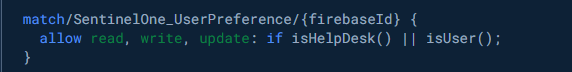
\includegraphics[width=0.8\textwidth]{Figures/User Preference.png}
  \caption{Granting access of read, write, and update from User Preference collection to users in the Firebase Console}
\end{figure}


\begin{lstlisting}[language=JavaScript, caption={Model class in the back-end}]
  export interface Customer {
  customerId: string;
  customerName: string;
  orgUnitType: string;
  parentId: string;
  city: string;
  stateProv: string;
  country: string;
  county: string | null;
  postalCode: string;
  contactEmail: string;
}

/**
 * Class for CustomerModel.
 */
export class CustomerModel {
  private readonly firestore: FirebaseFirestore.Firestore;
  private readonly collectionName = "customers";
  private readonly context = "CustomerModel";

  /**
   * Constructor for CustomerModel.
   */
  constructor() {
    this.firestore = admin.firestore();
  }

  /**
   * Serializes a Customer object to a JSON string.
   * @param {Customer} customer The Customer object to serialize.
   * @return {string} The serialized JSON string.
   */
  serializeCustomerToJson(customer: Customer): string {
    return JSON.stringify(customer);
  }

  /**
   * Deserializes a JSON string to a Customer object.
   * @param {string} json The JSON string to deserialize.
   * @return {Customer} The deserialized Customer object.
   */
  deserializeJsonToCustomer(json: string): Customer {
    return JSON.parse(json) as Customer;
  }

  /**
   * Creates a new customer in Firestore.
   * @param {Customer} customer Customer to add to Firestore.
   * @return {Promise<FirebaseFirestore.DocumentReference<FirebaseFirestore.DocumentData>> | undefined}.
   */
  async createCustomer(customer: Customer): Promise<FirebaseFirestore.DocumentReference<FirebaseFirestore.DocumentData> | undefined> {
    try {
      return this.firestore.collection(this.collectionName).add(customer);
    } catch (ex: unknown) {
      logError(ex, this.context + ".createCustomer");
    }
    return undefined;
  }

  /**
   * Retrieves a customer by its ID from Firestore.
   * @param {string} customerId The ID of the customer to retrieve.
   * @return {Promise<Customer | undefined>} A promise that resolves with the customer object if found, or undefined if not found or an error occurs.
   */
  async getCustomer(customerId: string): Promise<Customer | undefined> {
    try {
      const doc = await this.firestore.collection(this.collectionName).doc(customerId).get();
      if (!doc.exists) {
        return undefined;
      }
      return doc.data() as Customer;
    } catch (ex: unknown) {
      logError(ex, this.context + ".getCustomer");
      return undefined;
    }
  }

  /**
   * Updates an existing customer in Firestore.
   * @param {string} customerId The ID of the customer to update.
   * @param {Partial<Customer>} customer The partial customer object containing updates.
   * @return {Promise<void>} A promise that resolves when the update is complete.
   */
  async updateCustomer(customerId: string, customer: Partial<Customer>): Promise<void> {
    try {
      await this.firestore.collection(this.collectionName).doc(customerId).update(customer);
    } catch (ex: unknown) {
      logError(ex, this.context + ".updateCustomer");
    }
  }

  /**
   * Deletes a customer from Firestore.
   * @param {string} customerId The ID of the customer to delete.
   * @return {Promise<void>} A promise that resolves when the customer is successfully deleted.
   */
  async deleteCustomer(customerId: string): Promise<void> {
    try {
      await this.firestore.collection(this.collectionName).doc(customerId).delete();
    } catch (ex: unknown) {
      logError(ex, this.context + ".deleteCustomer");
    }
  }

}
\end{lstlisting}
\subsection{Setting up permissions with Firestore}

This has got to do with the Firestore database and the access level of permission that a Firebase Cloud Function has. In the
SentinelOne integration project, the table that contains SentinelOne data cannot be changed by the client, only by fetching new
data from the SentinelOne \acrshort{api} and replacing the old data. Therefore, only one table remains that can be
changed accordingly by the user, the User Preference table. This table can be changed freely by the user if they remain
logged in to the \acrshort{qaas} app.


\subsection{Connection to Algolia}

As originally stated, the author and Company Supervisor directly intended on using Algolia search as the SentinelOne
\acrshort{api} search, although far from being bad, does have type intolerance. The purpose of this is to enhance the \acrshort{ux}
because not all users can remember the exact name of the data they want to search for and makes the search more accurate and faster
even with false inputs.

\acrshort{qict} itself already has the test environment project set up in Algolia, because they are also using it in every search functionality
that they have in the \acrshort{qaas} app. For this specific project, the author's work \acrshort{qict} Microsoft e-mail account was invited to join
the project. In there, the author can already see all the duplicate indexes coming from Firestore that serves as the point of reverence when letting
the \acrshort{ai} Algolia engine to do the searching. From Algolia dashboard, several default \acrshort{api} keys can be seen, including:
\begin{itemize}
  \item Application \acrshort{id}: unique application identifier
  \item Search \acrshort{api} key: usable for search queries and for listing the indices.
  \item Write \acrshort{api} key: is used to create, update, and delete indices. Cannot be used to manage other \acrshort{api} keys.
  \item Admin \acrshort{api} key: like write keys but can be used to manage other \acrshort{api} keys.
\end{itemize}

The way the extension itself works is that it acts as a pre-written cloud function like Cloud Firestore Triggers (\textit{\cite{cloudTriggers}}),
where it listens to the collection in a Firestore. When the data changes this cloud function passes it through Algolia. It is a script Firebase made
together with Algolia. On this extension, 2 parameters are needed to be included: the Application \acrshort{id} and the \acrshort{api} key. The Application
\acrshort{id} is used to point to the right project in Algolia. The \acrshort{api} key is used to authenticate the connection between Algolia and Firebase.
For every Algolia extension, it is recommended to create a separate \acrshort{api} key and not to use the admin key, so that the key can be revoked if needed.
The author is using the custom \acrshort{api} key that was made by the Company Supervisor, that has restriction on the index that it can access, and the
operations that it can do.

% \begin{figure}[htbp]
%   \centering
%   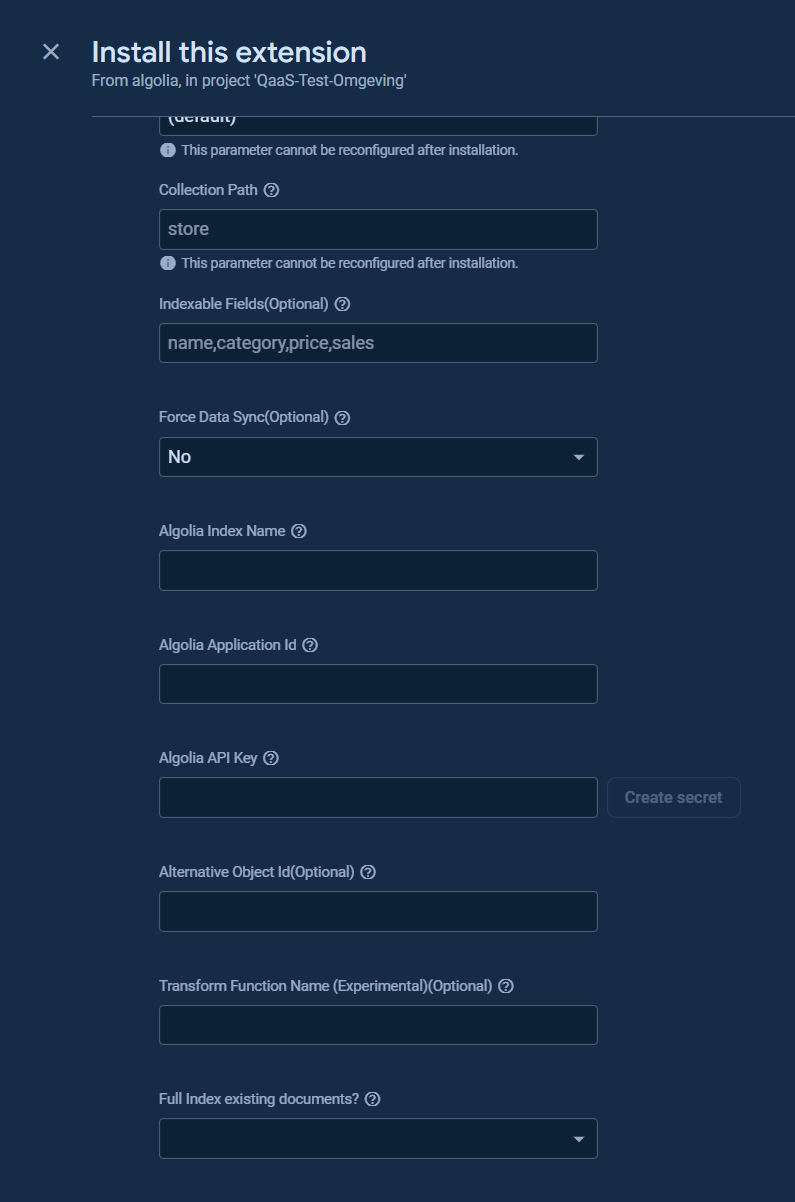
\includegraphics[width=0.8\textwidth]{Figures/Firebase Algolia Extension.png}
%   \caption{The Algolia configuration when installing the extension in the Firebase Console}
% \end{figure}

% \begin{figure}[htbp]
%   \centering
%   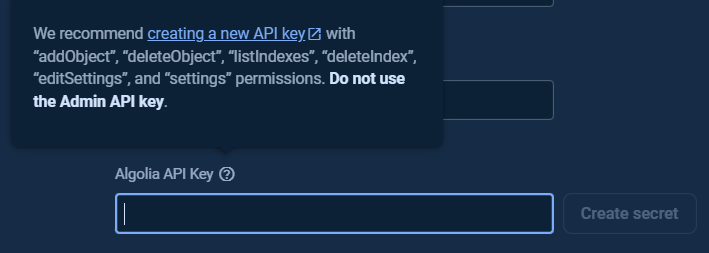
\includegraphics[width=0.8\textwidth]{Figures/Algolia API Key needed.png}
%   \caption{The Algolia \acrshort{api} key that is needed to be included in the Firebase Console when installing the extension}
% \end{figure}

% \begin{figure}[htbp]
%   \centering
%   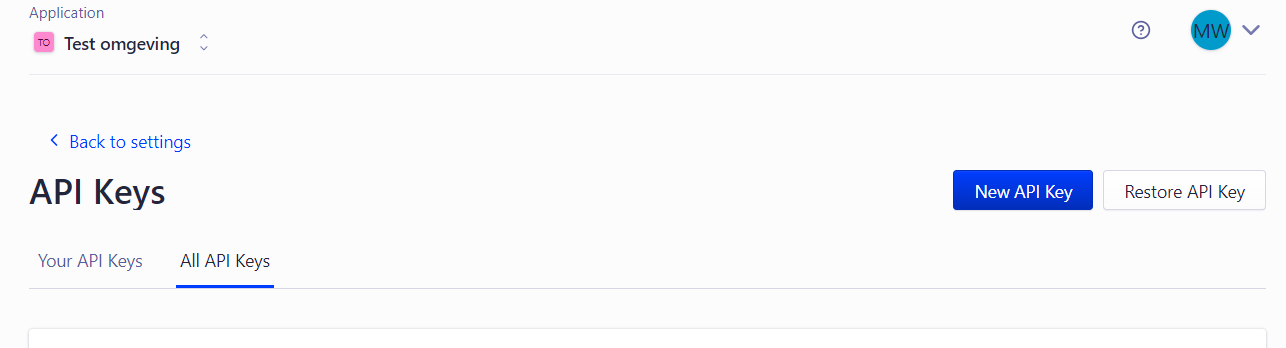
\includegraphics[width=0.8\textwidth]{Figures/Create new Algolia keys.png}
%   \caption{Creating a new Algolia key to use in the Firebase Extension}
% \end{figure}

% \begin{figure}[htbp]
%   \centering
%   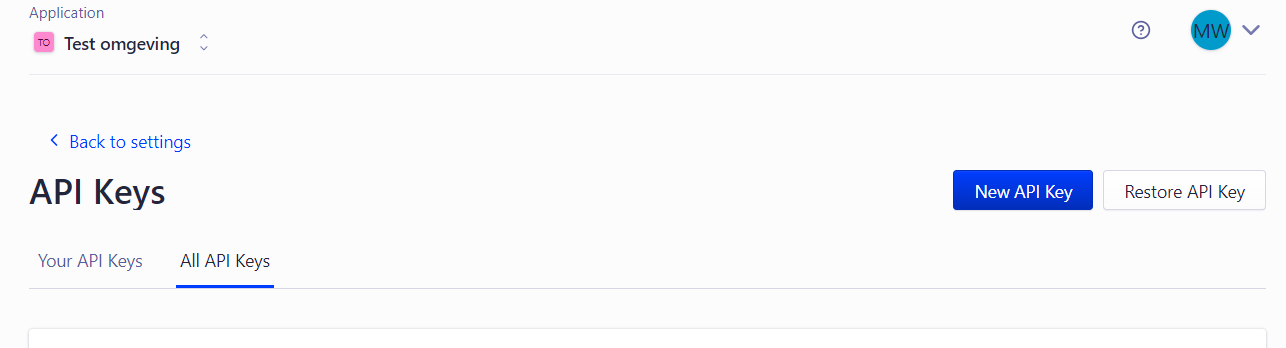
\includegraphics[width=0.8\textwidth]{Figures/Create new Algolia keys.png}
%   \caption{Creating a new Algolia key to use in the Firebase Extension}
% \end{figure}

% \begin{figure}[htbp]
%   \centering
%   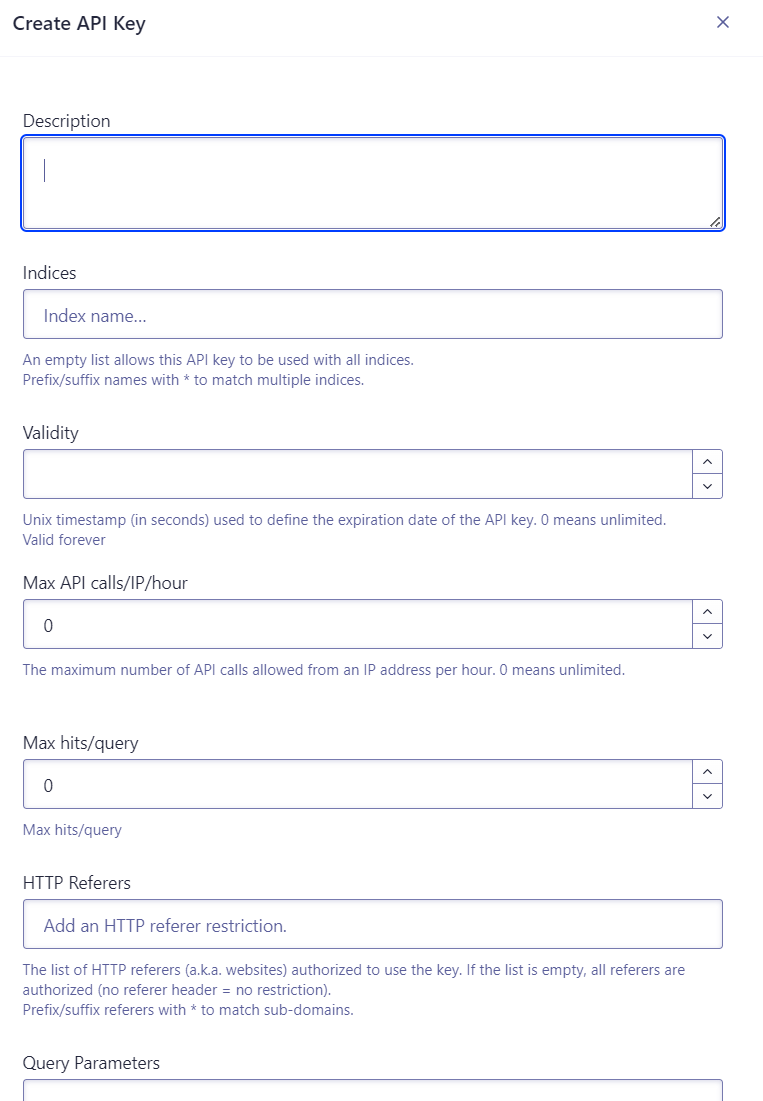
\includegraphics[width=0.8\textwidth]{Figures/Algolia API Key restrictions.png}
%   \caption{Algolia \acrshort{api} key restrictions that can be set up when creating a new key}
% \end{figure}

% \begin{figure}[htbp]
%   \centering
%   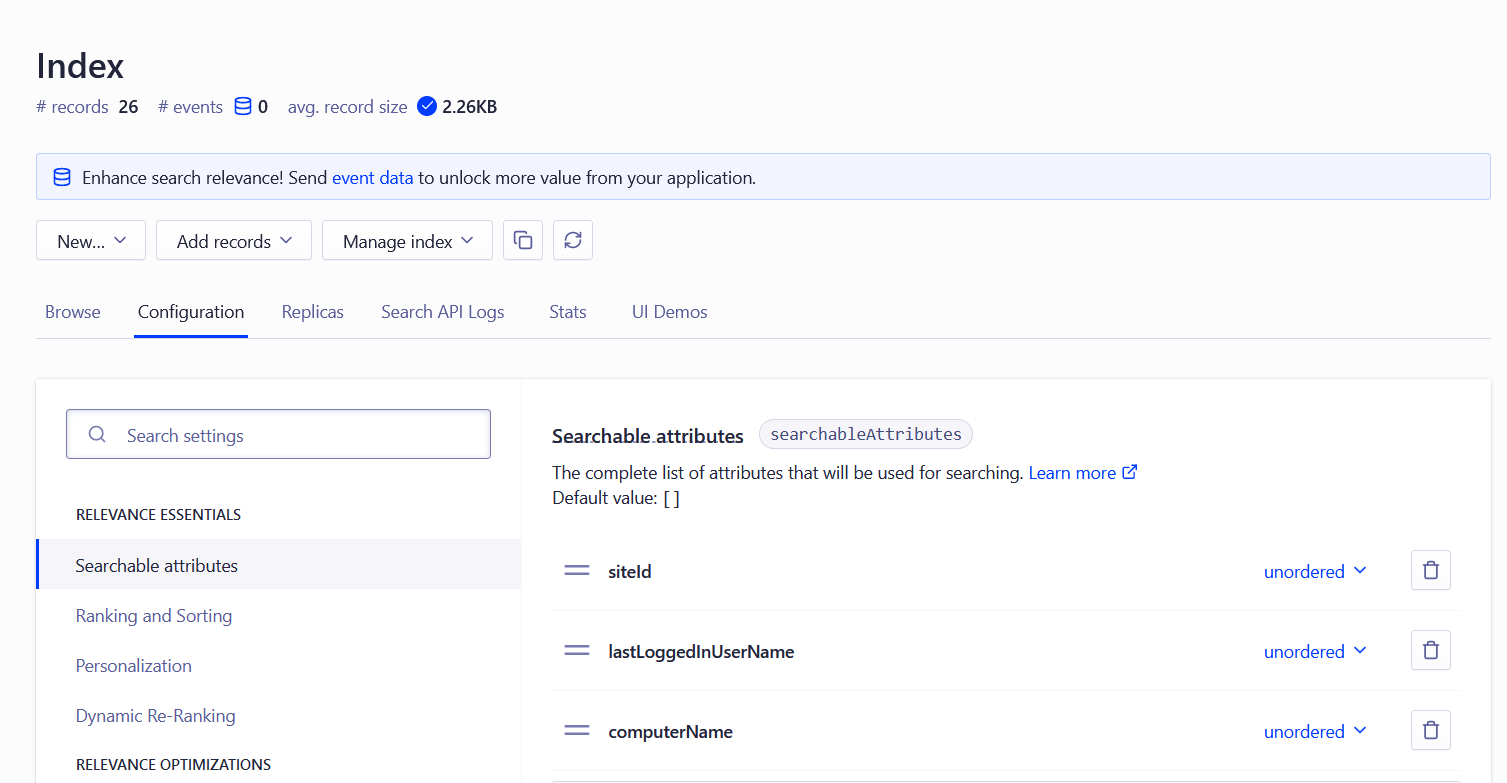
\includegraphics[width=0.8\textwidth]{Figures/Algolia Configuration.png}
%   \caption{All indexes need to have a configuration in which what searchable attributes that the user can search for, based on the
%     modelling of the JSON data structure}
% \end{figure}

\section{The Front-end}

In the front-end side of this project, it is just a matter of calling the Cloud Functions, modelling the \acrshort{json} response
coming from the Cloud Functions (whether it is from Firestore or SentinelOne), making the visualization graphs using the available
Flutter package, setting the logic on how to navigate between pages passing the correct data, the logic for how to display the data
correctly in paginated data tables and visualization widgets, and lastly, the searching, filtering, and filtering functionality.

After ensuring that the logic of the front-end works perfectly for showing the data, the last step that was needed to be undertaken
was polishing, which includes: checking for bugs and translation error, unit testing, making sure that the malfunctioning part that
were not yet fixed due to time constraint are not shown and testing for responsiveness on different devices. The last part was
proven to be quite a long process, because almost every widget that the author has created needed to be wrapped around another
Flexible widget that can expand and shrink based on the screen size, and to make sure that there is no infinity width or height
that can cause the widget to be cut off or not shown at all.

%   \subsubsection{Downloading PDF and HTML report files from SentinelOne to the client}

%   At almost the end of the realization phase, based on a work item requested by the stakeholders on the SCRUM board, the author has
%   decided to include showing the reports that have been made automatically or manually by SentinelOne or the cybersecurity actors
%   on \acrshort{qict}'s SentinelOne environment. The process initially was quite low on the priority list (Could have on the MOSCOW),
%   SentinelOne already has an \acrshort{api} that will give the \acrshort{ascii} characters of the \acrshort{pdf}, but calling this
%   directly on the client itself is not possible due to CORS blocking policy. Therefore, a Cloud Function is needed as a middleman
%   for getting the \acrshort{pdf} file to the client.

%   First on the back-end, when using \texttt{axios} to call the appropriate SentinelOne \acrshort{url}, another header needs to be
%   included to specify that the expected response format is \acrshort{pdf}. Additionally, the response type also need to be set
%   to \texttt{arraybuffer} to hand;e binary data efficiently.

%   Lastly, upon receiving the request, the binary data is converted into a base64-encoded string. This is necessary to ensure
%   that the binary data can be safely transmitted and displayed within the web client. Additionally, the content of the \acrshort{mime}
%   type of the response is extracted from the headers to facilitate proper handling of the data on the client side.

%   When the client accepts the response, it is necessary the base64-encoded string is decoded into a byte of array. Then, to facilitate
%   the download of the \acrshort{pdf}, a \texttt{Blob} is created from the decoded byte array. An object  \acrshort{url} is then
%   generated from this \texttt{Blob}, and an anchor element is programmatically created and clicked to trigger the download.

%   This way, a \acrshort{pdf} or \acrshort{html} file can be downloaded on the client side using any type of web browser when running the
%   \acrshort{qaas} app.


% \begin{lstlisting}[language=Dart, caption={How calling and modelling a response works in Flutter}]

%   class Data extends BaseModel {
%     Data({
%       required this.id,
%       required this.name,
%       required this.age,
%     });

%     factory Data.fromJson(Map<String, dynamic> json) {
%       return Data(
%         id: json['id'] as String,
%         name: json['name'] as String,
%         age: json['age'] as int,
%       );
%     }

%     final String id;
%     final String name;
%     final int age;

%     Map<String, dynamic> toJson() {
%       return {
%         'id': id,
%         'name': name,
%         'age': age,
%       };
%     }
%   }

%   static Future<List<Data>> getData() async {
%     try {
%       final HttpsCallable callable =
%           FirebaseFunctions.instanceFor(region: 'europe-west3').httpsCallable(
%         'getData',
%         options: HttpsCallableOptions(
%           timeout: const Duration(seconds: 540),
%         ),
%       );

%       final Map<String, dynamic> headers = <String, dynamic>{
%         'dataType': 'abcd',
%       };

%       final HttpsCallableResult<dynamic> results = await callable.call(headers);
%       final Map<String, dynamic> responseData =
%           results.data as Map<String, dynamic>;
%       final dynamic data = responseData['data'];

%       if (data is List<dynamic>) {
%         return data
%             .map((dynamic json) =>
%                 Data.fromJson(json as Map<String, dynamic>))
%             .toList();
%       } else if (data is Map<String, dynamic>) {
%         return <Data>[Data.fromJson(data)];
%       }
%     } on FirebaseFunctionsException catch(e) {
%       if (kDebugMode) {
%         print('Firebase error when fetching the data: $e');
%       }
%     } catch (e, stack) {
%       if (kDebugMode) {
%         print('Application error: $e \nStack: $stack');
%       }
%     }
%     return List<Data>.empty();
%   }
% \end{lstlisting}


% \begin{lstlisting}[language=JavaScript, caption={How downloading a PDF/HTML file works on the back-end}]
%   const response = await axios.get(urlName, {
%     headers: {
%       "Authorization": `ApiToken ${apiToken}`,
%       "Accept": "application/pdf",
%     },
%     responseType: "arraybuffer",
%   });

%   const answer = {
%     data: Buffer.from(response.data, "binary").toString("base64"),
%     contentType: response.headers["content-type"],
%   };

%   return { data: answer };
% \end{lstlisting}


% \begin{lstlisting}[language=Dart, caption={How downloading a PDF/HTML file works on the front-end}]
%   static Future<void> downloadPdfReports({
%     required String reportId,
%   }) async {
%     try {
%       final HttpsCallable callable =
%           FirebaseFunctions.instanceFor(region: 'europe-west3').httpsCallable(
%         'getReports',
%         options: HttpsCallableOptions(
%           timeout: const Duration(seconds: 540),
%         ),
%       );

%       final Map<String, dynamic> headers = <String, dynamic>{
%         'reportId': reportId,
%       };

%       final HttpsCallableResult<dynamic> results = await callable.call(headers);
%       final Map<String, dynamic> responseData =
%           results.data as Map<String, dynamic>;
%       final String base64Data = responseData['data'] as String;

%       // Decode the base64 string to bytes
%       final Uint8List bytes = base64Decode(base64Data);

%       // Create a Blob from the byte data
%       final html.Blob blob = html.Blob([bytes], 'application/pdf');

%       // Create an object URL from the Blob
%       final String url = html.Url.createObjectUrlFromBlob(blob);

%       // Create an anchor element and trigger a download
%       html.AnchorElement(href: url)
%         ..setAttribute('download', 'report.pdf')
%         ..click();

%       // Optionally revoke the Blob URL after some time to release resources
%       Future<void>.delayed(
%           const Duration(seconds: 5), () => html.Url.revokeObjectUrl(url));

%       if (kDebugMode) {
%         print('PDF download triggered');
%       }
%     } on FirebaseFunctionsException catch (ex) {
%       if (kDebugMode) {
%         print('Firebase error when downloading the PDF: $ex');
%       }
%     } catch (e, stack) {
%       if (kDebugMode) {
%         print('Application error: $e \nStack: $stack');
%       }
%     }
%   }
% \end{lstlisting}

\section{Deploying everything to the Live environment}

In the final phase of the project, after making sure that everything works and tested properly, the author needed to deploy the project
from the test environment to the live environment, so that other users can also access it. Below are the steps undertaken to deploy the
project to the live environment:

\begin{enumerate}
  \item Make sure to log in to the admin account of the Firebase Console.
  \item Make sure to select the right environment.
  \item Create a specific branch in the Azure DevOps repository for the live environment (live-\textit{date}).
  \item Switch the firebase options to the live environment in the Flutter new client.
  \item Make sure there are no debug app check tokens in the index.html of the Flutter project.
  \item Build the Flutter client project.
  \item Deploy the new Flutter client code to Firebase, now the front-end is updated.
  \item Add/ update/ delete any Firebase cloud functions for the new version to get added into the live environment.
  \item Create \acrshort{api} secrets in the live environment if needed.
  \item Allow secret access to the specific cloud functions.
  \item Make sure the Firebase security rules are up-to-date in the live environment.
  \item Mirror Cloud Firestore data in Algolia if needed.
  \item Change allowed Algolia indexes in Algoia \acrshort{api} key functions, this decides which indexes the developers
        are allowing to search on with this specific Algolia search \acrshort{api} key.
  \item Build Firestore indexes if needed, for where/ orderby queries, this is usually done before client deployment.
\end{enumerate}